\chapter{Experimental Setup}\label{chapter:experimental-setup}
This chapter explains the experiments in detail. How they are set up, where the data comes from and what exactly is measured and why. All the experiments in this thesis are designed in the Python programming language and evaluated on the same hard- and software configuration (cf. table \ref{tab:hardware}).
\begin{table}[H]
\centering
\begin{tabular}{@{}ll@{}}
\toprule
Processor          & 6 core Intel Core i7-6850K CPU @ 3.60GHz         \\
Memory             & 32GB                                             \\
Graphics Processor & $2\cross$ Geforce GTX 1080 8GB linked via NVLink \\
Operating System   & Ubuntu 16.04 LTS                                 \\
CUDA               & 9.0                                              \\
Python             & 3.6.6                                            \\
PyTorch            & 0.4.1                                            \\
BindsNET           & 0.1.8                                            \\ \bottomrule
\end{tabular}
\caption[Hardware and Software Components]{Hardware and software components used to run all the experiments.}
\label{tab:hardware}
\end{table}

\section{Neural networks}
The experiments are run on 4 different types of neural networks, that follow different paradigms and vary in their degree of biological plausibility. Namely they are:
\begin{enumerate}
    \item A classical 4-layer convolutional neural network.
    \item Vector capsules with dynamic routing in a 3-layer neural network.
    \item Convolutional matrix capsule layers as part of a 5-layer network.
    \item A shallow spiking neural network with a single hidden layer.
\end{enumerate}
The CNN, vector and matrix capsules are all implemented within the PyTorch \cite{paszke2017automatic} framework. This allows them to be trained using the same established optimization schemes. Spiking neural networks however require additional dynamics, that are not usually part of the typical tensor-based neural network software libraries. Therefore, the SNN used in the experiments is implemented on top of the recently released BindsNET \cite{2018arXiv180601423H}, a python package that extends PyTorch with the neural dynamics necessary for spiking neural networks and biological learning algorithms like STDP. The respective networks' topologies are determined largely by a mix of experience, published results on similar data as well as trial and error. However, due to the relative simplicity and low resolution of the used data, they are all shallow architectures, which makes it easier to draw conclusions about the used technology w.r.t their performance. Note that the following networks all include an input layer which is not explicitly listed. The input layer has always the same dimension as the input image.
\subsubsection{CNN}
As CNNs are generally well established a good network topology for the experiments could easily be found and comes down to a variation of a classical LeNet \cite{lecun1998gradient}. The network consists of 4 layers, with max pooling operations after each convolutional layer. For the exact network topology, see table \ref{tab:cnn-config}.
\begin{table}[H]
\centering
\begin{tabular}{@{}lll@{}}
\toprule
Layer                   & \multicolumn{2}{l}{Configuration} \\ \midrule
Convolutional layer 1   & Number of kernels   & 32          \\
                        & Kernel size         & $5\cross 5$ \\
                        & Stride              & 1           \\
                        & Activation function & ReLU        \\
Max pooling             & Window size         & $2\cross 2$ \\
Convolutional layer 2   & Number of kernels   & 64          \\
                        & Kernel size         & $5\cross 5$ \\
                        & Stride              & 1           \\
                        & Activation function & ReLU        \\
Max pooling             & Window size         & $2\cross 2$ \\
Fully connected layer 1 & Number of neurons   & 1024        \\
                        & Activation function & ReLU        \\
Fully connected layer 2 & Number of neurons   & 5           \\
                        & Activation function & Softmax     \\ \bottomrule
\end{tabular}
\caption[Layers of the convolutional neural network]{Layers of the convolutional neural network and their configuration, defining the entire network's topology. Note that the number of weights between the second convolutional layer and the first fully connected layer computes as the product of the number of total neurons in each layer, i.e. $\qty(64\cross 5\cross 5)\cross 1024 = \num{1638400}$}
\label{tab:cnn-config}
\end{table}
\subsubsection{Vector Capsules}
The vector capsule network is composed of 3 layers in total. This composition is the minimal configuration to run a capsule network and similar to the one used by Sabour et al. in 2017. Namely it is made up of a convolutional layer that is used to initialize the poses and activations of the primary capsule layer and the class capsule layer on top. However, other than the network used by Sabour et al., there is no decoder on top of the class capsule layer and no reconstruction loss is used to train the network. Instead, the vector capsule network is directly trained using the length of the output vector of the class capsules, similarly to the matrix capsule network by Hinton et al. This has the added benefit that the vector capsules can be trained using the exact same mechanism as the convolutional and matrix capsule networks. Also, the network is not forced to encode features, that are useful for reconstruction but rather encouraged to learn features, that are useful for correct classification. Additionally, compared to Sabour et al. the width of the convolutional layer, the vector output dimensionality as well as the kernel size of the primary capsules are reduced, without losing any accuracy. Together with the removal of the decoder, this greatly reduces the number of parameters to train (cf. table \ref{tab:vector-config}). Routing-by-agreement (cf. algorithm \ref{alg:routing-by-agreement}) is used between the capsule layers. The routing algorithm is implemented using PyTorch tensors and operators -- this makes it possible to efficiently run the network on GPUs and use the automatic gradients to train the part-whole matrices.
\begin{table}[H]
\centering
\begin{tabular}{@{}lll@{}}
\toprule
Layer               & \multicolumn{2}{l}{Configuration}     \\ \midrule
Convolutional layer & Number of kernels       & 32          \\
                    & Kernel size             & $5\cross 5$ \\
                    & Stride                  & 1           \\
                    & Activation function     & ReLU        \\
Primary capsules    & Number of capsule types & 32          \\
                    & Kernel size             & 1           \\
                    & Stride                  & 2           \\
                    & Dimensionality          & 14          \\
                    & Activation function     & Squash (cf. equation \ref{eq:squash}) \\
Class capsules      & Number of types         & 5           \\
                    & Input dimension         & 14          \\
                    & Output dimension        & 8           \\ \bottomrule
\end{tabular}
\caption[Layers of the vector capsule network]{Layers of the vector capsule network and their configuration. The network consists of 3 layers, only 2 of which are capsule layers. This represents the bare minimum for a capsule network, as one layer is required to initialize the primary capsules and routing is only possible between two consecutive capsule layers.}
\label{tab:vector-config}
\end{table}
\subsubsection{Matrix Capsules}
There is only little research published on matrix capsules to draw from. For this reason, the network topology is exactly the same as the \enquote{small} configuration used by Hinton et al., which they used for image data of the same size as in these experiments. Nevertheless, training matrix capsules is quite challenging, as the gradient will often either vanish or the capsules won't learn at all. To prevent this from happening, capsule-aware versions of dropout and batch normalization are implemented (cf. section \ref{sec:training}). They differ from the regular implementation by considering the internal representation of matrix capsules ($4\cross 4$ pose matrices and $2D$ feature activity maps). By respectively deactivating or normalizing highly correlated groups of neurons, the network can be regularized during training \cite{hinton2012improving}. All of the capsule layers are convolutional and comprised of matrix capsules (cf. table \ref{tab:matrix-config}).
\begin{table}[H]
\centering
\begin{tabular}{@{}lll@{}}
\toprule
Layer                    & \multicolumn{2}{l}{Configuration}                   \\ \midrule
Convolutional layer      & Number of kernels       & 64                        \\
                         & Kernel size             & $5\cross 5$               \\
                         & Stride                  & 2                         \\
                         & Padding                 & 2                         \\
                         & Activation function     & ReLU                      \\
Batch normalization      &                         &                           \\
Dropout                  &                         &                           \\
Primary capsules         & Number of capsule types & 8                         \\
                         & Kernel size             & $1\cross 1$               \\
                         & Stride                  & 1                         \\
                         & Dimensionality          & $4\cross 4$               \\
                         & Activation function     & Sigmoid (only activities) \\
Dropout                  &                         &                           \\
Convolutional capsules 1 & Number of capsule types & 16                        \\
                         & Kernel size             & $3\cross 3$               \\
                         & Stride                  & 2                         \\
                         & Dimensionality          & $4\cross 4$               \\
Dropout                  &                         &                           \\
Convolutional capsules 2 & Number of capsule types & 16                        \\
                         & Kernel size             & $3\cross 3$               \\
                         & Stride                  & 1                         \\
                         & Dimensionality          & $4\cross 4$               \\
Dropout                  &                         &                           \\
Class capsules           & Number of types         & 5                         \\
                         & Kernel size             & $1\cross 1$               \\
                         & Stride                  & 1                         \\
                         & Dimensionality          & $4\cross 4$               \\ \bottomrule
\end{tabular}
\caption[Layers of the matrix capsule network]{Layers of the matrix capsule network. Note that the matrix capsules include a $4\cross 4$ pose matrix as well as a logit representing the activation probability. As such they are comprised of 17 neurons each. Further note that only the size of the primary capsule kernels is given in pixels, while the others are given in whole capsules.}
\label{tab:matrix-config}
\end{table}\noindent
Expectation-Maximization routing (cf. algorithm \ref{alg:em-routing}) is employed between all adjacent capsule layers. As with vector capsules, automatic generation of gradients for the operations used inside the routing algorithm is utilized to train the part-whole matrices and description costs discriminatively.
\subsubsection{SNN}
In order to achieve a similar performance and allow comparison with the other networks, the SNN is designed to facilitate training using stochastic gradient descent with backpropagation. Input images are rate-encoded by setting the firing rate of the spiking neurons in the input layer proportional to the pixel-intensities. The error signal during training is then calculated by applying a softmax to the average firing rates of the second fully connected layer (cf. table \ref{tab:snn-config}). Although this is only an approximation as the firing rate is not differentiable w.r.t the synaptic weights, this approach achieves better classification performance than STDP-based learning with the same network.
\begin{table}[H]
\centering
\begin{tabular}{@{}lll@{}}
\toprule
Layer        & \multicolumn{2}{l}{Configuration} \\ \midrule
Fully connected layer 1 & Number of neurons      & TODO     \\
             & Neuron model           & LIF      \\
Fully connected layer 2 & Number of neurons      & 5        \\
             & Neuron model           & LIF      \\
             & Activation function    & Softmax  \\ \bottomrule
\end{tabular}
\caption[Layers of the spiking neural network]{Layers of the spiking neural network. All of the neurons are modelled as leaky integrate-and-fire neurons. Only a single hidden layer is used due to the expressiveness of spiking neurons. The softmax in the final layer is only applied to the average firing rates during exposure to the input and assumes the role of a loss function.}
\label{tab:snn-config}
\end{table}\noindent
Thanks to the BindsNET software package, spiking neural networks can be run on graphical processing units, same as the other network architectures. However, as there is no support for the automatic computation of gradients for networks of spiking neurons yet -- in BindsNET or any other framework -- the gradients have to be computed by hand and implemented directly. This somewhat limits the complexity of the available network's topology.
\subsubsection{Hyperparameters}
Because they have a huge influence over the respective network's performance, all the relevant hyperparameters are optimized in an exhaustive search. To this end, parameter candidates are arranged on a heuristically determined hypergrid with each axis corresponding to a hyperparameter. Each point on the hypergrid is trained and evaluated on a full object recognition dataset to find a good tuple of parameters (i.e. one that achieves high accuracy on a test set). The hyperparameters included in the search for the CNN, vector capsule and matrix capsule networks are explained in table \ref{tab:pytorch-hypers} as they use the same optimization scheme. For the SNN hyperparameters, see table \ref{tab:bindsnet-hypers}.
\begin{table}[H]
\centering
\begin{tabular}{@{}ll@{}}
\toprule
Parameter           & Description                                                  \\ \midrule
batch size         & Number of samples processed during a pass                     \\
learning rate      & Size of the step taken during gradient descent               \\
epochs             & Number of training epochs                                    \\
routing iterations & Iterations of dynamic routing, only used in capsule networks \\ \bottomrule
\end{tabular}
\caption[Hyperparameter definitions of the convolutional, vector capsule and matrix capsule networks]{Hyperparameter definitions of the convolutional, vector capsule and matrix capsule networks. Note that not all the hyperparameters are used by all the network architectures.}
\label{tab:pytorch-hypers}
\end{table}

% Please add the following required packages to your document preamble:
% \usepackage{booktabs}
% \usepackage{longtable}
% Note: It may be necessary to compile the document several times to get a multi-page table to line up properly
\begin{longtable}[c]{@{}ll@{}}
\toprule
Parameter      & Description                                                               \\* \midrule
\endfirsthead
%
\endhead
%
\bottomrule
\endfoot
%
\endlastfoot
%
hidden neurons & The number of neurons in the hidden layer                                 \\
time           & Length of time in milliseconds input is generated during training \\
learning rate  & Size of the step taken during gradient descent                            \\
decay rate     & Rate the learning rate is decayed by the scheduler                        \\
patience       & Number of intervals without progress before the scheduler                 \\
               & decays the learning rate                                                  \\
interval       & Size of an interval in number of samples processed                        \\
epochs         & Number of training epochs                                                 \\* \bottomrule
\caption[Hyperparameter definitions of the spiking neural network]{Hyperparameter definitions of the spiking neural network. Note that compared to common CNN schedulers, the learning rate can be decayed during an epoch.}
\label{tab:bindsnet-hypers}
\end{longtable}
\subsubsection{Training}
All of the networks are trained discriminatively by stochastic gradient descent (or a variation thereof) with backpropagation over several epochs. The CNN, vector and matrix capsules all employ the same optimization scheme. The scalar output of their final layer is used to compute spread loss (cf. equation \ref{eq:spread-loss}), which is minimized by PyTorch's implementation of the Adam algorithm \cite{kingma2014adam}. A scheduler is used, that decreases the learning rate by a factor of $\num{10}$ after each epoch of training, which doesn't increase accuracy on the training data. Additionally, the inverse temperature of the logistic function (cf. equation \ref{eq:matrix-logistic}) used in EM routing for the matrix capsules is adjusted on a linear schedule. The net result of this is that the sigmoidal shape of the logistic function becomes steeper over the epochs, effectively encouraging the routing to become more concise. The SNN on the other hand uses SGD computed based on the average firing rates of the output neurons with softmax as an error function. The inputs are generated by sampling for a fixed period of time from a Poisson distribution with the firing rate proportional to the pixels' intensities. Because of the asynchronous nature of spiking neurons, only a single training sample can be viewed at a time, compared to the other networks, that process a batch of input samples in parallel. A similar scheduler is implemented to decrease the learning rate, but greater care has to be taken w.r.t choosing the scheduler's hyperparameters as the training is more susceptible to changes in learning rate than the Adam algorithm.
\section{Datasets}\label{sec:datasets}
A virtual experiment for the Neurorobotics Platform (NRP) is designed to create object recognition data. Experiments for the NRP consist of a virtual environment, one or more robots and a brain based on spiking neural networks that can be connected to the robot's sensors and actuators via so-called transfer functions \cite{knoll2016neurorobotics}. The environment in this experiment is fairly simple, it consists of a plane, several objects and a number of different lights. A digital clone of an iCub robot \cite{vannucci2015visual} is placed into the environment and presented each object (cf. figure \ref{fig:nrp}).
\begin{figure}[H]
    \centering
    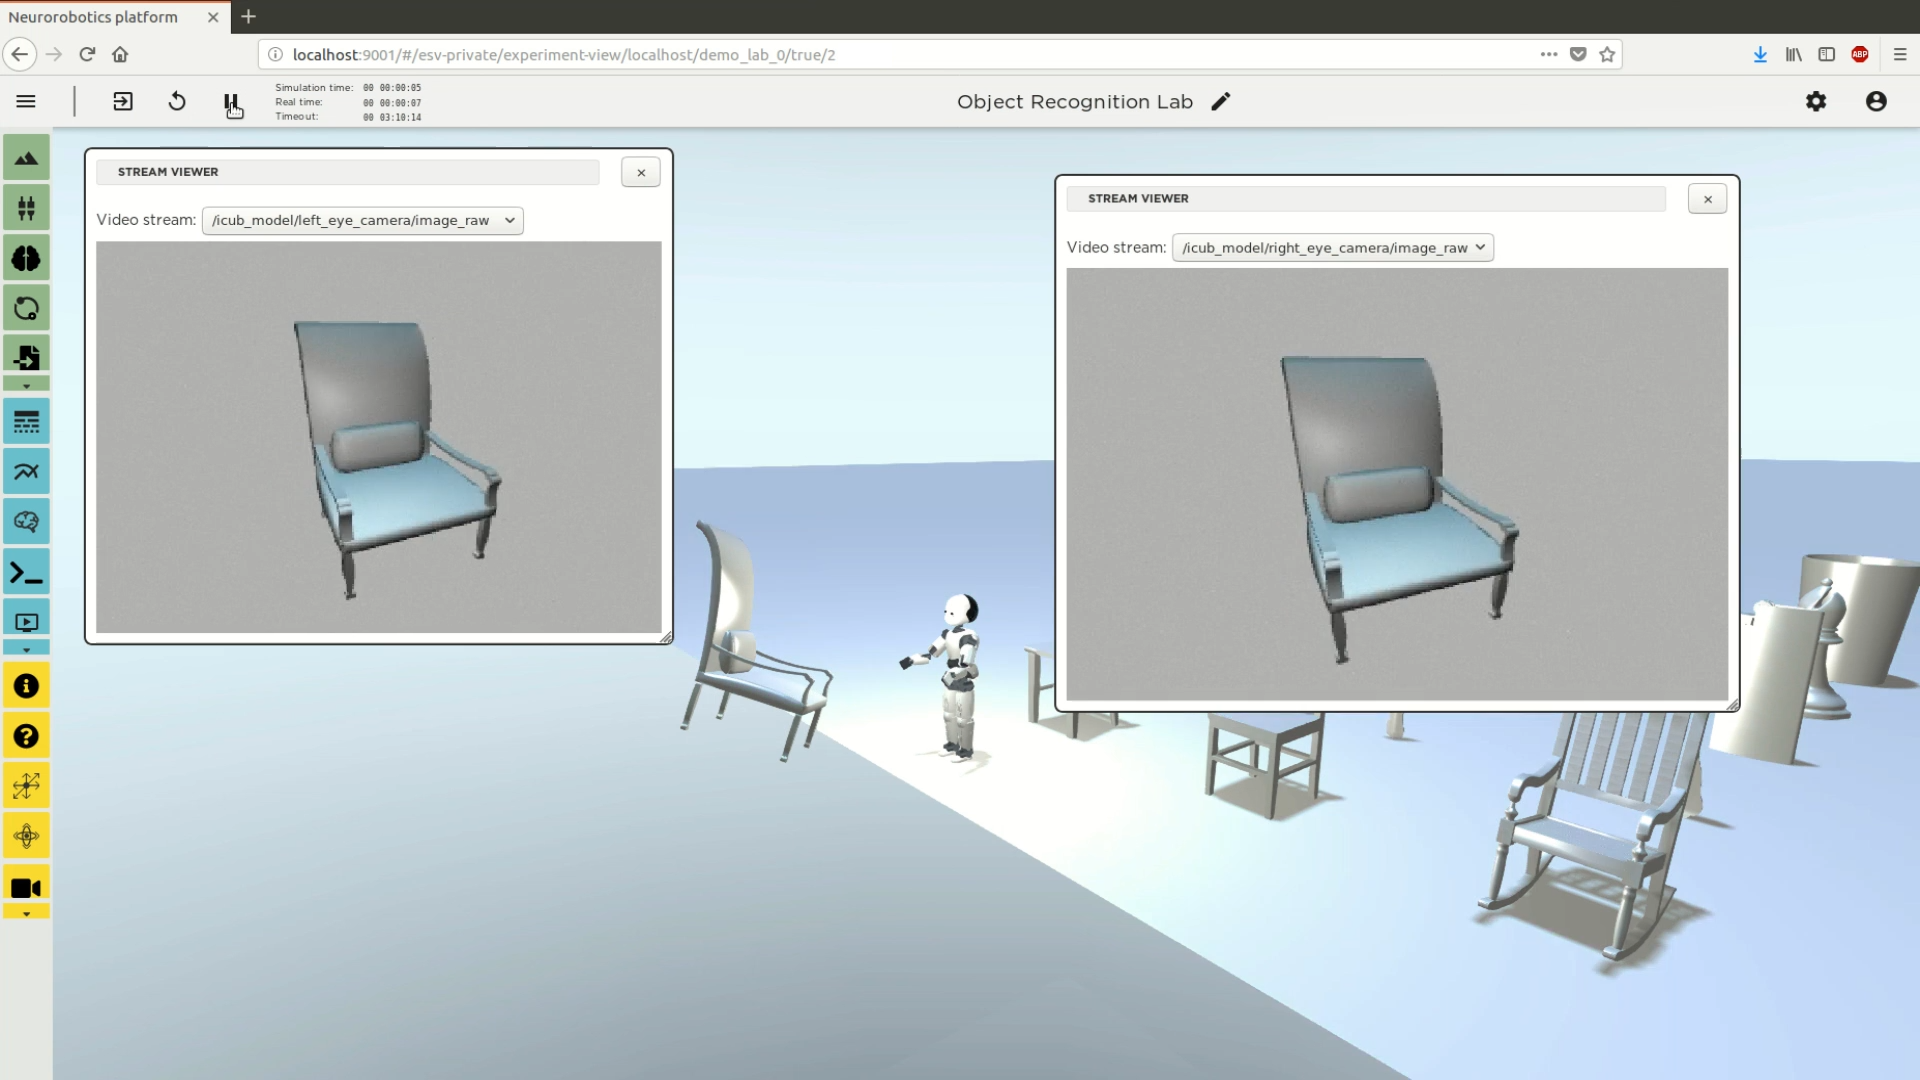
\includegraphics[width=\textwidth]{figures/nrp.png}
\caption[Screenshot of the Neurorobotics Experiment creating object recognition data.]{Screenshot of the Neurorobotics Experiment creating object recognition data. The Experiment is viewed from inside a browser. Note that each of the two windows is a live view of one of the iCub robot's video cameras placed in its eyes. Thus, realistic and to scale stereo images can be generated.}\label{fig:nrp}
\end{figure}\newpage\noindent
The objects are presented from different viewpoints and under varying lighting conditions, while the NRP handles physical simulation and rendering of the scene. This includes simulation of the robot's noisy sensors, which can be queried for their data. In this case, the iCub's video cameras are used to capture stereo images from the iCub's point of view. The captured images can then be grouped into datasets and trained on the different neural network architectures. Each image includes labels describing the class the viewed object belongs to, the lighting conditions as well as the viewpoint. In total, there are 8 different objects of 5 classes each. They are designed to represent everyday household items, such as future robots may need to recognize (cf. figure \ref{fig:dataset}).
\begin{figure}[H]
    \centering
    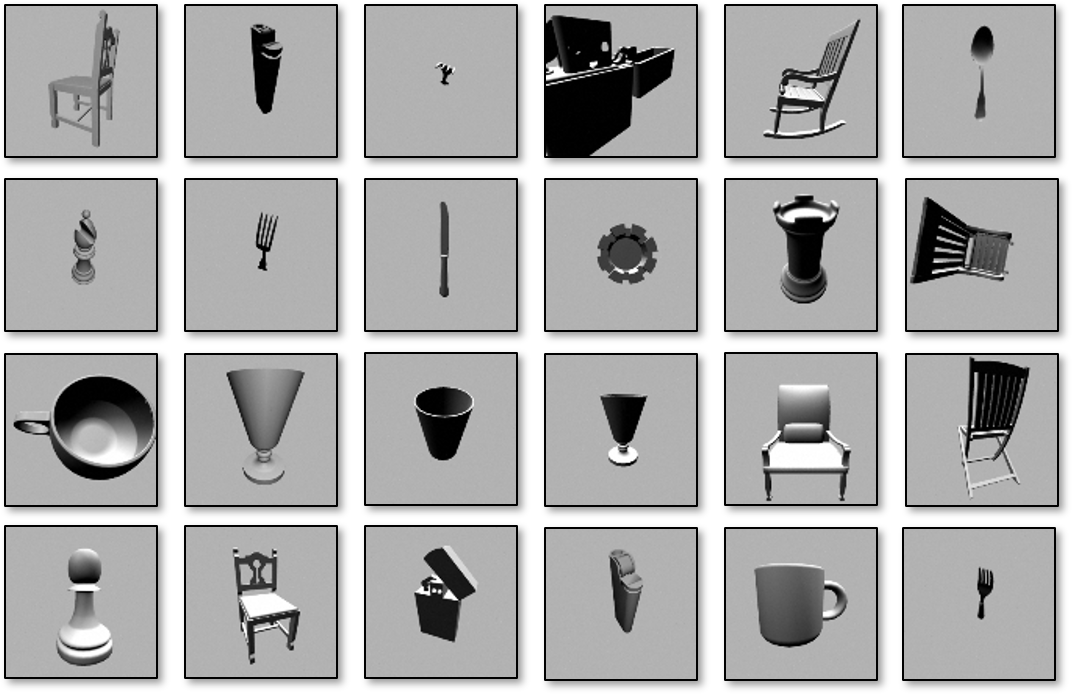
\includegraphics[width=\textwidth]{figures/dataset.png}
\caption[Samples from the object recognition dataset.]{Samples from the object recognition dataset. The 5 classes are chairs, chess figures, cutlery, cups and lighters. Each class consists of 8 objects, that are viewed from 162 different viewpoints under 4 distinct lighting-setups. Note that while the objects obviously vary in shape they also vary in topology,  e.g. there are cups with and without a handle or chairs standing on 4 legs compared to rocking chairs.}\label{fig:dataset}
\end{figure}\noindent
As matrix capsules were specifically conceived by Hinton et al. as shape recognition units to learn part-whole relationships, the datasets are designed with an emphasis on shape recognition. As such they do not feature any textures or colors. However, they are still very challenging object recognition tasks. Outliers that vary greatly in shape as well as topology were deliberately included. The rationale behind this is, that while there is some variance within a class, the classes still differ enough from each other, such that a good recognition system should be able to rule out false positives. While the lighting can be varied continuously, 4 different setups are chosen, that vary in the number, direction and intensity of lights in the scene. The different viewpoints are taken from a solid angle of size $2\pi\,\si{\steradian}$, i.e. the upper half-dome with the object at the center, discretely sampled at 9 elevations and 18 azimuths for a total of 162 points. However, rather than moving the entire robot, only the object is rotated. Specifically, the lights are not rotated with the object. Compared to similar datasets, this results in complex interactions between the lights and the object (cf. figure \ref{fig:viewpoint}).
\begin{figure}[H]
    \centering
    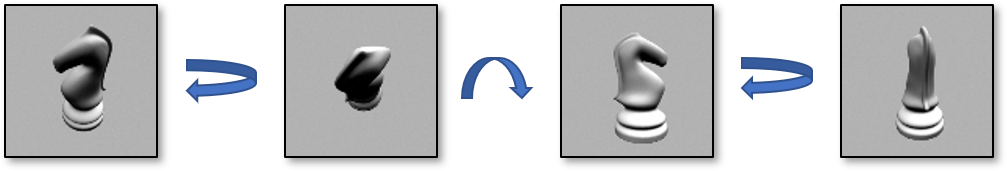
\includegraphics[width=\textwidth]{figures/viewpoint.png}
\caption[Samples of different viewpoints from the object recognition dataset.]{Samples of different viewpoints from the object recognition dataset. The same object from the class of chess figures is viewed from different azimuths and elevations under the same lighting. Note that while the shape of the figure is symmetrical across one axis, the two sides are lit-up differently under different viewpoints.}\label{fig:viewpoint}
\end{figure}\noindent
Based on the basis dataset (consisting of all the objects, viewpoints and 4 different lighting setups) different augmented versions are created. These augmentations can be used as additional test sets for networks trained on the basis dataset to evaluate their capabilities further. To investigate how proficient the networks are at explaining-away perturbations in the form of occlusions, the datasets are incrementally augmented. Small geometric primitives that vary in shape, color and size are randomly placed on top of the objects until they cover a fixed percentage of the image (cf. figure \ref{fig:occlusion}).
\begin{figure}[H]
    \centering
    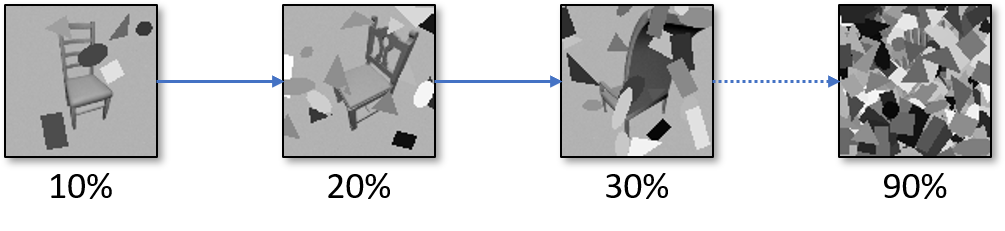
\includegraphics[width=\textwidth]{figures/occlusion.png}
\caption[Augmentation of the object recognition dataset to test for robustness against occlusion]{Augmentation of the object recognition dataset to test for robustness against occlusion. Ellipses, rectangles and triangles of varying shape and color are randomly placed on the images to occlude the object. An entire dataset is created for each increment in the percentage of coverage.}\label{fig:occlusion}
\end{figure}\newpage\noindent
Another augmentation of the datasets is intended to test for robustness of part-whole relationships. Capsule networks specifically are only supposed to activate the capsules in higher levels, if the capsules in the lower layers agree about the higher capsule's pose based on the pose of their own features. Classifiers that don't learn part-whole relationships could for example still activate as long as the parts are present, even if their pose is not consistent with the whole. By dividing each image into square tiles and randomly switching them, the location of features is effectively permuted on an even grid (cf. figure \ref{fig:picasso}). An argument can be made that the difficulty of testing for part-whole relationships increases with the number of tiles, because for fewer (i.e. bigger) tiles there are both bigger features and locally consistent submanifolds of features that agree.
\begin{figure}[H]
    \centering
    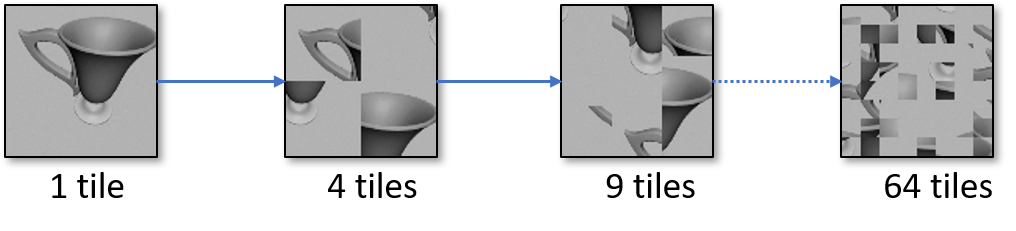
\includegraphics[width=\textwidth]{figures/picasso.png}
\caption[Augmentation of the object recognition dataset to test the robustness of part-whole relationships]{Augmentation of the object recognition dataset to test the robustness of part-whole relationships. The images are divided into an increasing number of squares that are randomly permuted. For each number of tiles, an entire dataset is created.}\label{fig:picasso}
\end{figure}\noindent
\section{Metrics}
The metrics used to evaluate the neural networks can be divided into runtime and classification metrics. The former deals with resource requirements needed to run the networks while the latter looks at their statistical performance as classifiers in object recognition tasks.
\subsubsection{Runtime Metrics}
To allow comparison of the runtime metrics, all the networks are trained for one epoch on the basic version of the object recognition dataset using the same batch size (i.e. practically normalizing time and memory measurements over batch size). This means training only one sample at a time, because the spiking neural network is unable to process mini batches. During training the memory allocated by the network and its computation graph is measured as well as the number of parameters that need to be trained and the time required to train the entire epoch. Latency of the trained networks is then measured by simply timing inference on the test set. Also, during inference, the memory requirements are measured again. Finally, to quantify the benefits of parallel processing on GPUs, the networks are again timed during training and inference using mini batches of the sizes determined by the hyperparameter grid search.
\subsubsection{Classification Metrics}
The most obvious classification metric is accuracy, i.e. the fraction of correct predictions during inference over the test set.
\begin{align}
    \operatorname{accuracy}\qty(\vb{Y}, \vb{T}) &= \frac{1}{\abs{T}}\sum_{i=1}^{\abs{T}} \mathbbm{1}\qty(y_i=t_i)
\end{align}
With $\vb{Y}=\qty(y_1,y_2,...)^T$ and $\vb{T}=\qty(t_1,t_2,...)^T$ containing the classifier's estimate of the training samples and the true class labels respectively and $\mathbbm{1}$ the indicator function. Information about all of the network's predictions in relation to the true labels can be neatly expressed within the so-called \emph{confusion matrix}. In a confusion matrix each row corresponds to the true class labels and each column to the prediction. Each entry is then the number of samples of class $i$ predicted to be class $j$ (cf. figure \ref{fig:confusion}).
\begin{align}
    M_{i,j} = \sum_{k=1}^{\abs{T}}\mathbbm{1}\qty(t_k = i)\mathbbm{1}\qty(y_k = j)
\end{align}
\begin{figure}[H]
    \centering
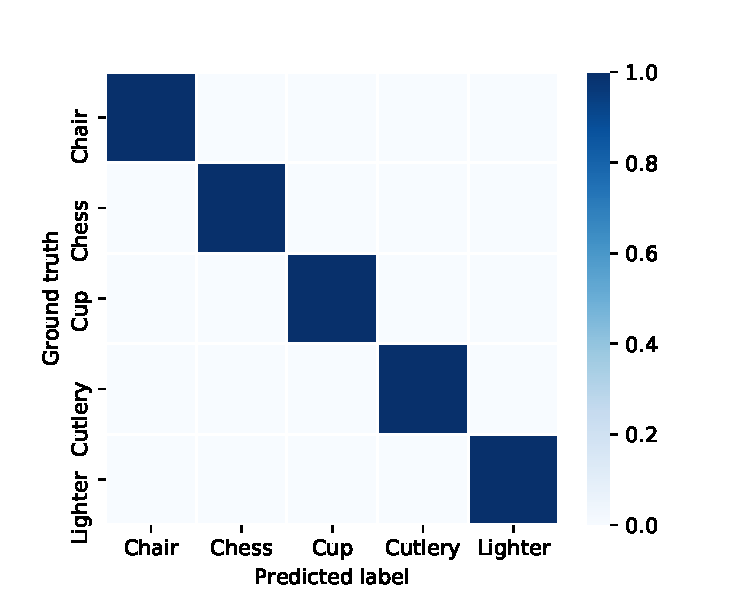
\includegraphics[clip,trim=0 0 0 1.1cm,width=.75\textwidth]{figures/confusion_matrix.pdf}
\caption[Example of a confusion matrix by means of a perfect classifier]{Example of a confusion matrix by means of a perfect classifier. The confusion matrix is plotted in the form of a heatmap for easy inspection of the accuracy across different classes. Note that a perfect classifier results in a diagonal matrix as the off-diagonal elements correspond to misclassifications.}\label{fig:confusion}
\end{figure}\noindent
For binary classifiers it is interesting to know the \emph{true positive rate} as well as the \emph{false positive rate}, i.e. the fraction of positive predictions that were correctly classified and the fraction of negative samples that were falsely classified as positive respectively. This information can be visualized by plotting the true positive rate against the false positive rate at various classification thresholds. The resulting curve is known as a \emph{receiver operating characteristic} (ROC) curve. It can be interpreted as depicting the trade-off between reward (true positives) and cost (false positives). The ROC space is divided by a diagonal into points representing good classifications above and predictions worse than random below (cf. figure \ref{fig:roc}). The curve information can be compiled into a single scalar value representing expected performance by computing the area under the curve (AUC). The ROC AUC of a classifier is equivalent to the probability that the classifier will rank a randomly chosen positive instance higher than a randomly chosen negative instance \cite{fawcett2006introduction}.
\begin{figure}[H]
    \centering
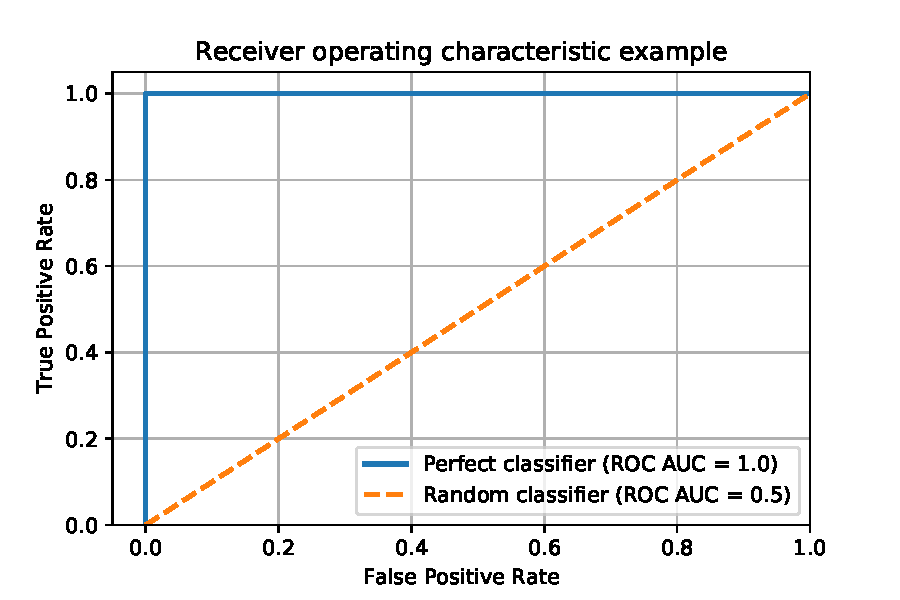
\includegraphics[clip,trim=0 0 0 1.1cm,width=.75\textwidth]{figures/roc.pdf}
\caption[Example of a ROC curve by means of a perfect classifier]{Example of a ROC curve by means of a perfect classifier. The curve of a perfect classifier always yields a true positive rate of $\SI{100}{\percent}$, while a random guess produces as many true as false positives and therefore corresponds to a diagonal. A real classifier will lie somewhere between those curves, i.e. the closer the ROC curve to the upper left corner of ROC space, the better the classifier.}\label{fig:roc}
\end{figure}\noindent
To evaluate the neural networks used in these experiments, the ROC is extended to multi-label classifiers. This is done by binarizing the output (one label is interpreted as positive while all others are negative, i.e. one-vs-all classification) and generating one ROC curve per class. All the ROC curves are then averaged to generate a single curve as well as AUC score \cite{provost2000well}.\newpage\noindent
Finally, a metric is used that fully leverages the versatility of the generated data from the Neurorobotics Platform to evaluate a network's ability to generalize. To test generalization, the networks are trained on a basic version of the data and tested on a perturbed version. The perturbed versions include the augmented data (occlusions and tiles respectively, cf. section \ref{sec:datasets}) but also viewpoints that are not explicitly trained. However, simply measuring the established metrics on a perturbed dataset only yields a single data point or point estimate of the network's ability to generalize. Instead, the \enquote{extent} of the perturbation across perturbation space can be parameterized to introduce a latent variable.
\begin{align}
     P_{\mathrm{Perturb}}\qty(\vb{t}\mid \vb{x},\vb*{\theta}) &= \int_{\Omega} P\qty(\vb{t}\mid \vb{x},\vb*{\theta},\vb*{\tau}) P\qty(\vb*{\tau}) \dd{\vb*{\tau}}
\end{align}
Where the sum and product rules of probability are used along with $\vb*{\tau}$ the perturbation parameter and $\Omega$ the perturbation space. By sampling $\vb*{\tau}$ from the prior distribution $P\qty(\vb*{\tau})$ the integral can be computed using Monte Carlo integration.
\begin{align}
    \int_{\Omega} P\qty(\vb{t}\mid \vb{x},\vb*{\theta},\vb*{\tau}) P\qty(\vb*{\tau}) \dd{\vb*{\tau}} \approx \frac{1}{T} \sum_{t=1}^T P\qty(\vb{t}\mid \vb{x},\vb*{\theta},\vb*{\tau}_t)
\end{align}
Using this formalism, the generalization is then expressed by the difference between the metrics of the unperturbed and the perturbed networks. The latter is computed by stochastically sampling from the parameterized perturbation space and computing the average of the metric evaluated on all samples. The augmented datasets are already parameterized. Another parameterized dataset can be created by incrementally removing random viewpoints from the training set and adding them to the test set. Use of Monte Carlo integration is justified as both the prior distribution of the latent variable is known (its uniform as it's generated in even increments) and the micro perturbations are generated stochastically. The generalization metrics determined this way should then be more informative than a single evaluation.